
\documentclass[../main.tex]{subfiles}

\begin{document}

Results of the query generation experiment are shown in Table \ref{tbl_results}.

\begin{table}[h!]
    \small
    \centering
    
\documentclass[../main.tex]{subfiles}

\begin{document}

Results of our evalution are shown in Table \ref{tbl_results}.

\begin{table}[h!]
    \small
    \centering
    
\documentclass[../main.tex]{subfiles}

\begin{document}

Results of our evalution are shown in Table \ref{tbl_results}.

\begin{table}[h!]
    \small
    \centering
    
\documentclass[../main.tex]{subfiles}

\begin{document}

Results of our evalution are shown in Table \ref{tbl_results}.

\begin{table}[h!]
    \small
    \centering
    \input{tables/results}
    \caption{}
    \label{tbl_results}
\end{table} 

\begin{figure}[h!]
  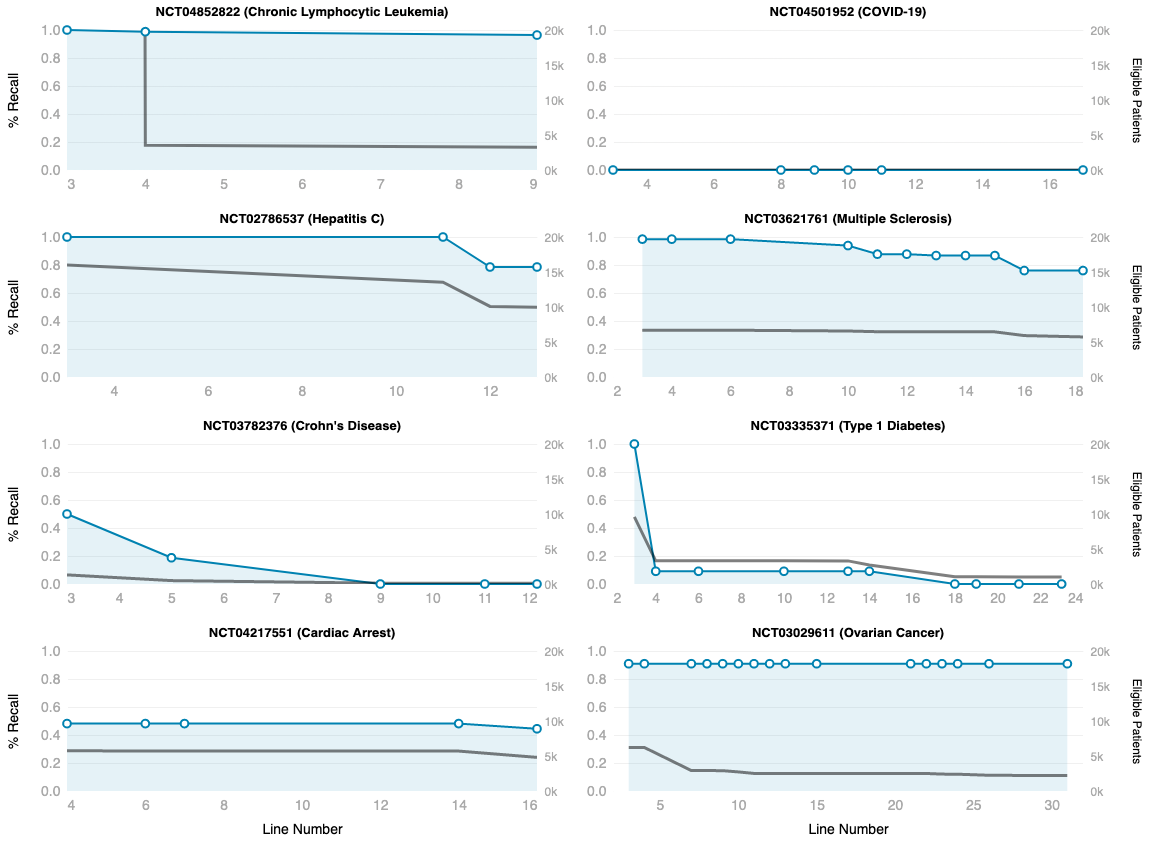
\includegraphics[scale=0.42]{figures/leafai_detail_results_longitudinal.png}  
\caption{}
\label{fig_leafai_results_longitudinal}
\end{figure}

\begin{table}[h!]
    \small
    \centering
    \input{tables/results_leafai_detail}
    \caption{}
    \label{tbl_results_leafai_detail}
\end{table} 


\end{document}
    \caption{}
    \label{tbl_results}
\end{table} 

\begin{figure}[h!]
  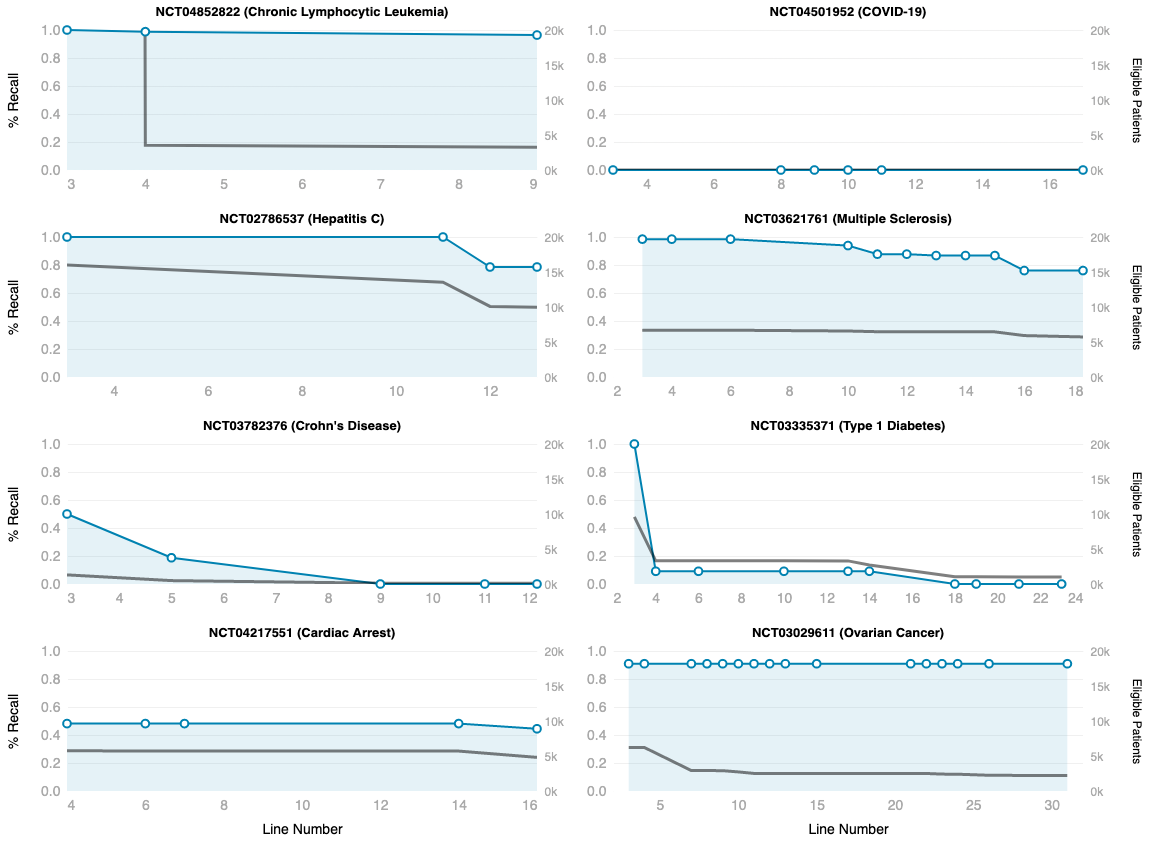
\includegraphics[scale=0.42]{figures/leafai_detail_results_longitudinal.png}  
\caption{}
\label{fig_leafai_results_longitudinal}
\end{figure}

\begin{table}[h!]
    \small
    \centering
    \def\arraystretch{1.4}
\begin{tabular}{l c c c c}
    \textbf{Condition} & \textbf{\# Criteria} & \textbf{Skipped - \newline No Patients} & \textbf{Skipped - \newline Not Computable} & \textbf{Fully Executed} \\
    \toprule
    Cl Lymphoma        & 4  & 0 (0\%)    & 0 (0\%)    & 4  (100\%)  \\
    Hepatitis C        & 8  & 0 (0\%)    & 4 (50\%)   & 4  (50\%)   \\
    Crohn's Disease    & 9  & 0 (0\%)    & 4 (44.4\%) & 5  (55.5\%) \\
    Cardiac Arrest     & 12 & 0 (0\%)    & 8 (66.6\%) & 4  (33.3\%) \\
    COVID-19           & 13 & 0 (0\%)    & 6 (46.1\%) & 7  (53.8\%) \\
    Multiple Sclerosis & 14 & 1 (7.1\%)  & 3 (21.4\%) & 10 (71.4\%) \\
    Type 1 Diabetes    & 18 & 2 (11.1\%) & 8 (44.4)   & 8  (44.4\%) \\
    Ovarian Cancer     & 25 & 2 (8\%)    & 9 (36\%)   & 14 (56\%)   \\
    \bottomrule
    \textbf{Total} & 103 & 5 (4.8\%) & 42 (40.7\%) & 61 (59.3\%)
\end{tabular}
    \caption{}
    \label{tbl_results_leafai_detail}
\end{table} 


\end{document}
    \caption{}
    \label{tbl_results}
\end{table} 

\begin{figure}[h!]
  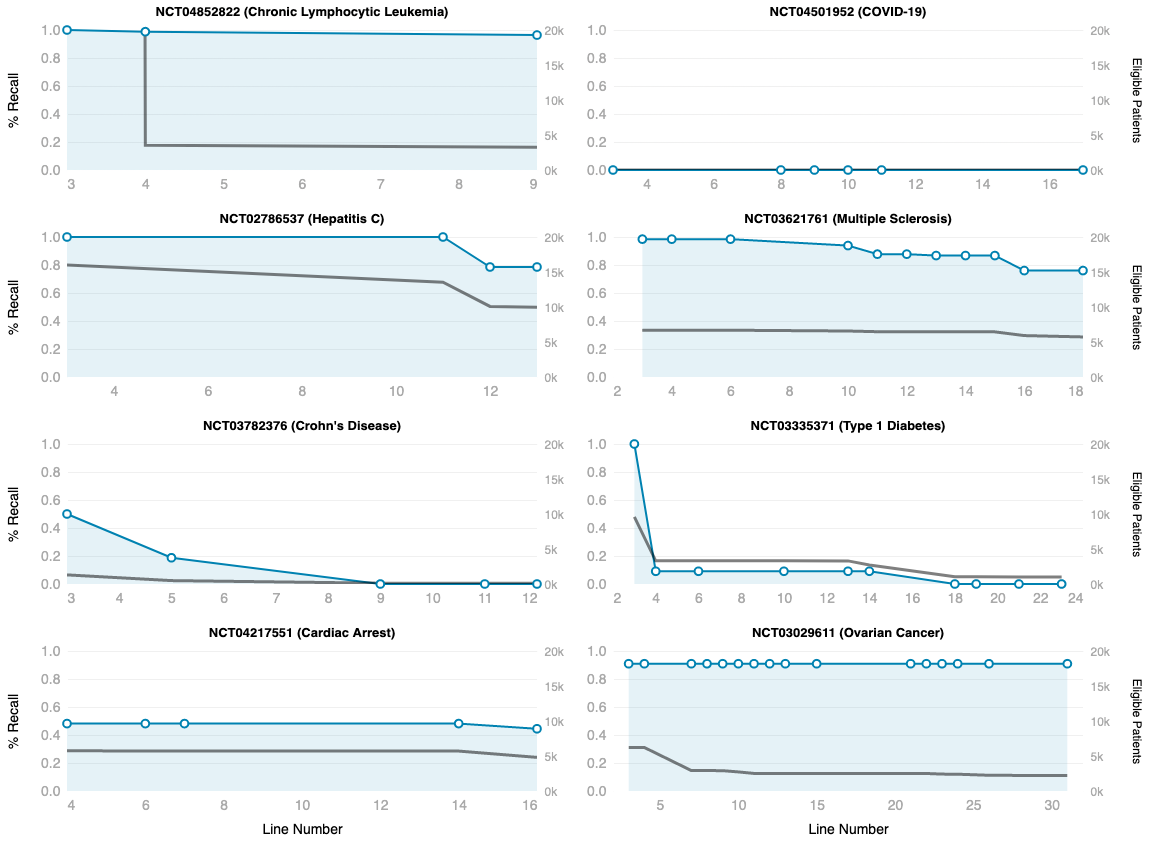
\includegraphics[scale=0.42]{figures/leafai_detail_results_longitudinal.png}  
\caption{}
\label{fig_leafai_results_longitudinal}
\end{figure}

\begin{table}[h!]
    \small
    \centering
    \def\arraystretch{1.4}
\begin{tabular}{l c c c c}
    \textbf{Condition} & \textbf{\# Criteria} & \textbf{Skipped - \newline No Patients} & \textbf{Skipped - \newline Not Computable} & \textbf{Fully Executed} \\
    \toprule
    Cl Lymphoma        & 4  & 0 (0\%)    & 0 (0\%)    & 4  (100\%)  \\
    Hepatitis C        & 8  & 0 (0\%)    & 4 (50\%)   & 4  (50\%)   \\
    Crohn's Disease    & 9  & 0 (0\%)    & 4 (44.4\%) & 5  (55.5\%) \\
    Cardiac Arrest     & 12 & 0 (0\%)    & 8 (66.6\%) & 4  (33.3\%) \\
    COVID-19           & 13 & 0 (0\%)    & 6 (46.1\%) & 7  (53.8\%) \\
    Multiple Sclerosis & 14 & 1 (7.1\%)  & 3 (21.4\%) & 10 (71.4\%) \\
    Type 1 Diabetes    & 18 & 2 (11.1\%) & 8 (44.4)   & 8  (44.4\%) \\
    Ovarian Cancer     & 25 & 2 (8\%)    & 9 (36\%)   & 14 (56\%)   \\
    \bottomrule
    \textbf{Total} & 103 & 5 (4.8\%) & 42 (40.7\%) & 61 (59.3\%)
\end{tabular}
    \caption{}
    \label{tbl_results_leafai_detail}
\end{table} 


\end{document}
    \caption{Statistics for each clinical trial evaluated by the LeafAI query engine and human programmer. The number of enrolled and matched patients were determined by cross-matching enrollments listed within our EHR.}
    \label{tbl_results}
\end{table} 

\begin{figure}[h!]
  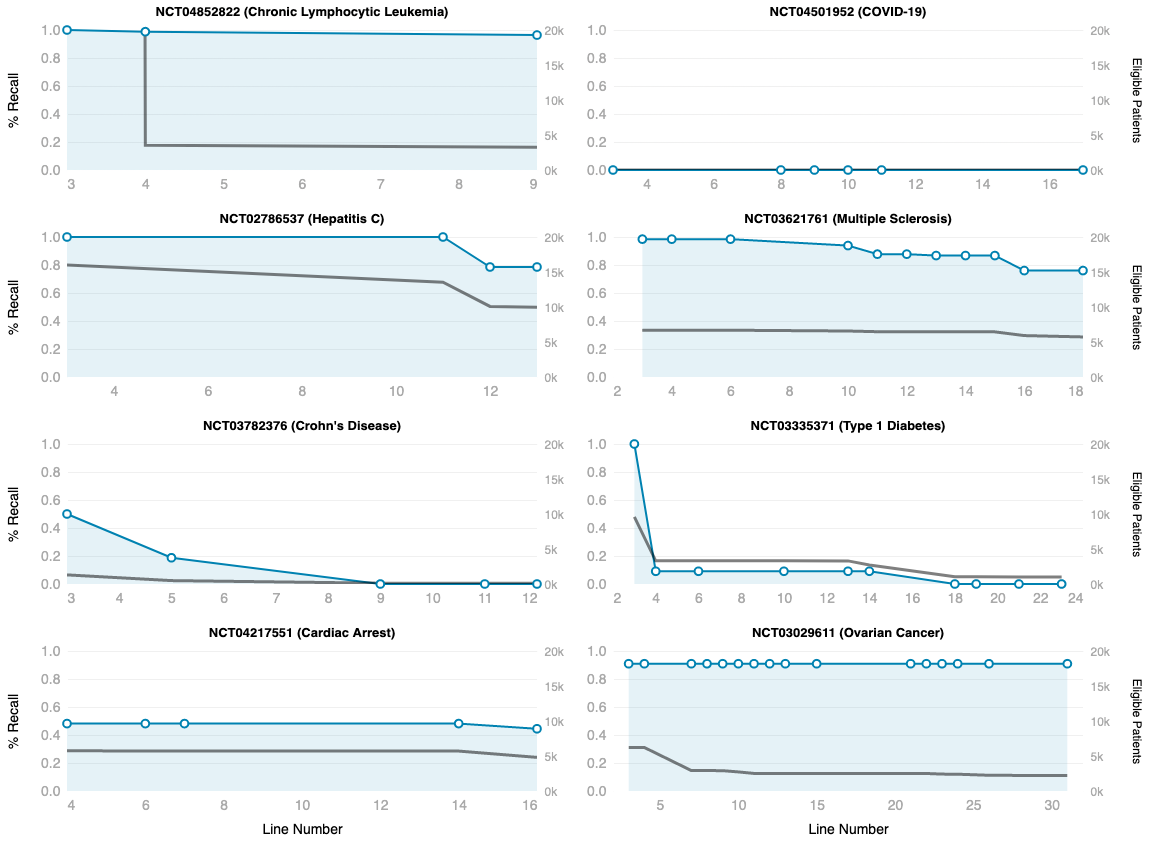
\includegraphics[scale=0.42]{figures/leafai_detail_results_longitudinal.png}  
\caption{Longitudinal results listing results of patients found at each step in the query process for each trial. The blue line indicates \% Recall (left-most Y axis) while the gray line indicates the number of eligible patients found (right-most Y axis). The X axis represents the line number within the free-text eligibility criteria. Dots indicate that the LeafAI query engine executed an eligibility criterion query.}
\label{fig_leafai_results_longitudinal}
\end{figure}

\begin{table}[h!]
    \small
    \centering
    \def\arraystretch{1.4}
\begin{tabular}{l c c c c}
    \textbf{Condition} & \textbf{\# Criteria} & \textbf{Skipped - \newline No Patients} & \textbf{Skipped - \newline Not Computable} & \textbf{Fully Executed} \\
    \toprule
    Cl Lymphoma        & 4  & 0 (0\%)    & 0 (0\%)    & 4  (100\%)  \\
    Hepatitis C        & 8  & 0 (0\%)    & 4 (50\%)   & 4  (50\%)   \\
    Crohn's Disease    & 9  & 0 (0\%)    & 4 (44.4\%) & 5  (55.5\%) \\
    Cardiac Arrest     & 12 & 0 (0\%)    & 8 (66.6\%) & 4  (33.3\%) \\
    COVID-19           & 13 & 0 (0\%)    & 6 (46.1\%) & 7  (53.8\%) \\
    Multiple Sclerosis & 14 & 1 (7.1\%)  & 3 (21.4\%) & 10 (71.4\%) \\
    Type 1 Diabetes    & 18 & 2 (11.1\%) & 8 (44.4)   & 8  (44.4\%) \\
    Ovarian Cancer     & 25 & 2 (8\%)    & 9 (36\%)   & 14 (56\%)   \\
    \bottomrule
    \textbf{Total} & 103 & 5 (4.8\%) & 42 (40.7\%) & 61 (59.3\%)
\end{tabular}
    \caption{The LeafAI query engine's handling of eligibility criteria for each trial. The column \textit{Skipped - No Patients} indicates the count of criteria which would, if executed, cause no patients to be eligible. The column \textit{Skipped - Not Computable} indicates the count of criteria which LeafAI could not generate a query for, for various reasons. Both of these types of criteria were ignored by the system.}
    \label{tbl_results_leafai_detail}
\end{table} 

\end{document}